\documentclass[10pt]{article}
\usepackage[margin=1in]{geometry}
\usepackage{amsmath,amssymb,amsthm}
\usepackage{booktabs}
\usepackage{array}
\usepackage{microtype}
\usepackage{url}
\urlstyle{tt}
\usepackage{tikz}
\usetikzlibrary{arrows.meta,positioning}
\usepackage{float}
\usepackage{enumitem}
\setlist{nosep}
\renewcommand{\arraystretch}{0.93}
\usepackage[hidelinks]{hyperref}
\setlength{\emergencystretch}{2.5em}

\newtheorem{theorem}{Theorem}[section]
\newtheorem{lemma}[theorem]{Lemma}
\newtheorem{proposition}[theorem]{Proposition}
\newtheorem{definition}[theorem]{Definition}
\newtheorem{corollary}[theorem]{Corollary}
\theoremstyle{remark}
\newtheorem{remark}[theorem]{Remark}
\theoremstyle{plain}

\newcommand{\NCh}{\mathit{ch}}
\newcommand{\Ncyc}{\mathit{cyc}}
\newcommand{\crit}{\operatorname{crit}}
\newcommand{\rot}{\operatorname{rot}}
\newcommand{\sig}{\operatorname{sig}}
\newcommand{\slack}{\operatorname{slack}}
\newcommand{\waste}{\operatorname{waste}}
\newcommand{\prog}[1]{\texttt{#1}}

\title{The shortest superpermutation on six symbols has\\length 872:
a concise proof}
\author{Worasait Suwannik\thanks{The research reported here was directed by Worasait Suwannik.  The proofs and the programs were produced by Claude, Anthropic's AI model.}}
\date{September 2026}

\begin{document}
\maketitle

\begin{abstract}
A superpermutation on $n$ symbols is a string containing every
permutation of the symbols as a contiguous window, and $M(n)$ is the
least length of one.  We prove that no superpermutation on six symbols
has length $871$ or less; with the known string of length $872$ this
gives an independent proof that $M(6)=872$.  An exact
accounting identity turns length $871$ into a structural budget.
Counting constraints valid for every superpermutation force a candidate
of that length to have zero slack and place it in one of sixteen
structural classes.  Exhaustive, independently cross-checked searches
then show that every class is empty.  The result is computer assisted:
every
computational step is carried by a named program in an accompanying
artifact repository, and the whole computational core re-runs on one
laptop inside a working day.
\end{abstract}

\section{Introduction}\label{sec:intro}

A \emph{superpermutation} on the alphabet $\{1,\dots,n\}$ is a string
over that alphabet containing each of the $n!$ permutations as a window
of $n$ consecutive characters, and $M(n)$ is the least length of such a
string.  The string $121$ shows $M(2)\le 3$ and $123121321$ shows
$M(3)\le 9$, and both are optimal.  The problem was posed by Ashlock
and Tillotson~\cite{AT93}, whose recursive construction gives
$M(n)\le 1!+2!+\cdots+n!$ and who conjectured that bound exact: it
holds for $n\le 5$, where $M(1),\dots,M(5)=1,3,9,33,153$, the last
value settled by the exhaustive search of Chaffin~\cite{C14}, and it
fails at $n=6$, where Houston~\cite{Houston14} produced in 2014 a
superpermutation of length $872$ against the conjectured $873$, so
$M(6)\le 872$.  The survey of Engen and Vatter~\cite{EV21} is the peer-reviewed
account of the classical background and of the earlier lower bounds.

Whether $872$ was optimal remained open for more than a decade.  The general lower
bound of the anonymous 4chan poster, Houston, Pantone and
Vatter~\cite{HPV18}, $M(n)\ge n!+(n-1)!+(n-2)!+n-3$, which is
Theorem~2.5 of~\cite{EV21}, gives $M(6)\ge 867$; Houston's improvement
by one, recorded in the remark following that theorem, gives
$M(6)\ge 868$.  In 2026 Raudvere~\cite{R26} gave a machine-checked
Lean~4 proof of $M(6)\ge 868$, the first publicly available
machine-checked proof of Houston's $+1$, and Hunter and Raudvere~\cite{HR26} a machine-checked general
bound giving $M(6)\ge 869$.  The residual gap consists of the lengths
$869$, $870$ and $871$, and is the gap addressed here.

Fritsch~\cite{Fritsch21} announced a proof of minimality on the
Superpermutators mailing list in 2021, pairing a lower-bound argument
with a search at length $871$; the public record describes that proof
as unfinished and, to our knowledge, no completed version has
appeared, so we do not treat the announcement as a completed proof.  The strategy followed here, a structural lower bound
sharpened until an exhaustive elimination at length $871$ becomes
affordable, is the same one.  In 2026 the question drew a
computer-assisted proof package~\cite{A6872repo}, developed by a
different group on a different decomposition, and a mailing-list
thread~\cite{SPML26} announcing a Lean-verified candidate.  The present
work was developed independently of both.

The work was carried out in three phases.  In the first, the model that
produced the proofs and the programs had no network access and worked
from the definitions alone; the searches, the classification and the
closure-topology theorem were complete and had passed an internal
adversarial review chain by 4 September 2026.  In the second, the author
relayed three rounds of external referee reports; in response the
proofs of the scanner inequalities, the cycle-shape exclusion and the
coverage theorem were written out in the form given here.  In the third,
from 7 September, the author supplied the package~\cite{A6872repo} with
its paper.  Its literature review is the source of the priority chain
and of the citations~\cite{R26,HR26}; its published length-872 witness
is the external control of Section~\ref{sub:scanner}; and its list of
open obligations prompted the clean-room second implementation of the
loop-mode search and the second derivation of the one certified capacity
value.  The thread~\cite{SPML26} was shown on 8 September as an index
entry.  No mathematical statement in this paper derives from either.

The argument reduces the existence of a length-$871$ superpermutation
to the acceptance of finitely many exhaustive searches, and the
reduction itself is carried by lemmas proved from the definitions, all
of which are given here.  A
structural class is called \emph{empty} when no first-occurrence
ordering whatsoever lies in it, not merely when some search failed to
find one; every emptiness claim in this paper is of that universally
quantified kind, and that is what makes an exhausted search a proof.
The programs, run logs and certificates are in an artifact
repository~\cite{REPO}, and Section~\ref{sec:programs} documents each
program in turn.

\section{From strings to a single finite question}\label{sec:reduction}

\begin{theorem}[Main Theorem]\label{thm:main}
No superpermutation on $\{1,\dots,6\}$ has length at most $871$; that
is, $M(6)\ge 872$.
\end{theorem}

\begin{proposition}[Upper bound]\label{prop:upper}
$M(6)\le 872$.
\end{proposition}

\begin{proof}
Houston~\cite{Houston14} exhibits a superpermutation on six symbols of
length $872$.  Such a string is a certificate, checked by sliding a
width-$6$ window along it and counting the distinct windows that are
permutations; one is shipped as
\prog{data/\allowbreak best872.txt} in~\cite{REPO} and checked in under
a minute by the program of Section~\ref{sub:checker}.
\end{proof}

\begin{corollary}\label{cor:main}
$M(6)=872$.
\end{corollary}

The proof of Theorem~\ref{thm:main} occupies
Sections~\ref{sec:reduction} to~\ref{sec:empty}, and
Figure~\ref{fig:map} is its map.  This section turns the theorem into
one finite question about one length.

\begin{figure}[H]\centering
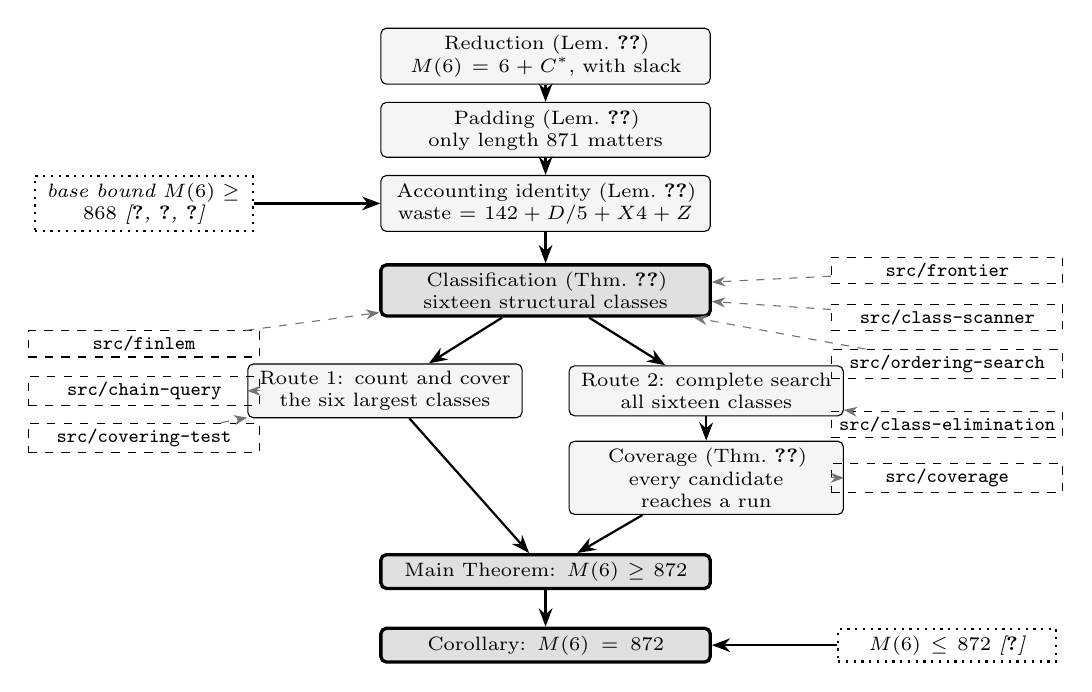
\begin{tikzpicture}[
  x=0.85mm, y=0.85mm,
  thm/.style={draw, rounded corners=2pt, align=center, inner sep=2.6pt,
              font=\scriptsize, fill=black!4, text width=40mm},
  key/.style={draw, rounded corners=2pt, align=center, inner sep=2.6pt,
              font=\scriptsize, fill=black!12, text width=40mm,
              very thick},
  rt/.style={draw, rounded corners=2pt, align=center, inner sep=2.6pt,
             font=\scriptsize, fill=black!4, text width=33mm},
  lit/.style={draw, dotted, thick, align=center, inner sep=2.4pt,
              font=\scriptsize\itshape, text width=26mm},
  prog/.style={draw, dashed, align=center, inner sep=2pt,
               font=\scriptsize\ttfamily, text width=28mm},
  arr/.style={-{Stealth}, thick},
  parr/.style={-{Stealth}, dashed, black!55}]

\node[thm] (red) at (0,0)    {Reduction (Lem.~\ref{lem:reduction})\\
                              $M(6)=6+C^{*}$, with slack};
\node[thm] (pad) at (0,-11)  {Padding (Lem.~\ref{lem:padding})\\
                              only length $871$ matters};
\node[thm] (acc) at (0,-22)  {Accounting identity
                              (Lem.~\ref{lem:identities})\\
                              $\waste=142+D/5+X4+Z$};
\node[key] (cls) at (0,-35)  {Classification (Thm.~\ref{thm:classes})\\
                              sixteen structural classes};
\node[rt]  (r1)  at (-24,-50){Route 1: count and cover\\
                              the six largest classes};
\node[rt]  (r2)  at (24,-50) {Route 2: complete search\\
                              all sixteen classes};
\node[rt]  (cov) at (24,-63) {Coverage (Thm.~\ref{thm:coverage})\\
                              every candidate reaches a run};
\node[key] (main) at (0,-77) {Main Theorem: $M(6)\ge 872$};
\node[key] (cor) at (0,-88) {Corollary: $M(6)=872$};

\node[lit] (base) at (-60,-22) {base bound $M(6)\ge 868$
                                \cite{HPV18,EV21,R26}};
\node[lit] (up)   at (60,-88) {$M(6)\le 872$ \cite{Houston14}};

\node[prog] (pfr) at (60,-32) {src/frontier};
\node[prog] (psc) at (60,-39) {src/class-scanner};
\node[prog] (pos) at (60,-46) {src/ordering-search};
\node[prog] (pce) at (60,-55) {src/class-elimination};
\node[prog] (pco) at (60,-63) {src/coverage};
\node[prog] (pfi) at (-60,-43) {src/finlem};
\node[prog] (pcq) at (-60,-50) {src/chain-query};
\node[prog] (pct) at (-60,-57) {src/covering-test};

\draw[arr] (red) -- (pad);
\draw[arr] (pad) -- (acc);
\draw[arr] (acc) -- (cls);
\draw[arr] (base) -- (acc);
\draw[arr] (cls) -- (r1);
\draw[arr] (cls) -- (r2);
\draw[arr] (r2)  -- (cov);
\draw[arr] (r1)  -- (main);
\draw[arr] (cov) -- (main);
\draw[arr] (main) -- (cor);
\draw[arr] (up)  -- (cor);
\draw[parr] (pfr) -- (cls);
\draw[parr] (psc) -- (cls);
\draw[parr] (pos) -- (cls);
\draw[parr] (pce) -- (r2);
\draw[parr] (pco) -- (cov);
\draw[parr] (pfi) -- (cls);
\draw[parr] (pcq) -- (r1);
\draw[parr] (pct) -- (r1);
\end{tikzpicture}
\caption{How the pieces connect.  Shaded boxes are the statements this
paper proves, the two heavy ones being the principal results;
dotted boxes are taken from the literature; dashed boxes are the
programs of Section~\ref{sec:programs}, attached by dashed arrows to
the statement whose exhaustive enumeration they carry.  The upper
bound enters only at the corollary, so the whole spine below the
reduction is the lower bound.}
\label{fig:map}
\end{figure}
\subsection{The reduction}


\begin{definition}\label{def:d}
For \emph{distinct} permutations $p\ne q$ of $\{1,\dots,6\}$, written
as six-letter words, let $d(p,q)$ be $6$ minus the length of the
longest suffix of $p$ that is also a prefix of $q$.  Since $p\ne q$
that suffix is proper, so $d(p,q)\in\{1,\dots,6\}$, and $d(p,q)$ is the
number of characters that must be appended after an occurrence of $p$
to produce an occurrence of $q$.  The \emph{overlap graph} has the
$720$ permutations as vertices and an arc $p\to q$ of weight $d(p,q)$
for each ordered pair of distinct permutations.
\end{definition}

The overlap graph and the reduction are Houston's~\cite[Section~2]{Houston14};
what Lemma~\ref{lem:reduction} adds is the exact treatment of the
inequality gaps.

\begin{lemma}[Reduction]\label{lem:reduction}
$M(6)=6+C^{*}$, where $C^{*}$ is the minimum weight of a Hamiltonian
path in the overlap graph.  Moreover every superpermutation $S$, whose
length we write $|S|$, induces an ordering $q_1,\dots,q_{720}$ of the
permutations, by position of first occurrence, with
\[
|S| \;=\; 6+\sum_{k=1}^{719} d(q_k,q_{k+1})+\slack(S),
\qquad \slack(S)\ge 0,
\]
and conversely gluing any ordering $q_1,\dots,q_{720}$ by maximal
overlap yields a superpermutation of length exactly $6+\sum d$, whose
own first-occurrence ordering need not be the one glued.
\end{lemma}

\begin{proof}
Gluing an ordering by maximal overlap gives a superpermutation of
length exactly $6+\sum d$, so $M(6)\le 6+C^{*}$.  Conversely, listing
the permutations of $S$ by first-occurrence position $p_k$, the string
must spell out enough of $q_{k+1}$ after $q_k$ to complete it, so
$p_{k+1}-p_k\ge d(q_k,q_{k+1})$; summing, with the six characters
before the first window ends and those after the last, gives the
identity with $\slack(S)$ collecting the gaps, and $|S|\ge 6+C^{*}$.
\end{proof}

\subsection{The padding argument}

\begin{lemma}[Padding]\label{lem:padding}
If no superpermutation on $\{1,\dots,6\}$ has length exactly $871$,
then none has length at most $871$.
\end{lemma}

\begin{proof}
Append $871-|S|$ arbitrary characters to a superpermutation $S$ of
length below $871$; every window of $S$ is still a window of the
result, which is therefore a superpermutation of length exactly $871$.
\end{proof}

\subsection{First-occurrence structure}

Fix a superpermutation $S=s_1s_2\cdots s_m$ over $\{1,\dots,6\}$, so
that its windows are the strings $s_i s_{i+1}\cdots s_{i+5}$ for
$1\le i\le m-5$, and let $q_1,\dots,q_{720}$ be its first-occurrence
ordering, with costs $d_k=d(q_k,q_{k+1})$.  Define
\[
\rot(p)=p_2p_3p_4p_5p_6p_1,\qquad
\sig(p)=p_3p_4p_5p_6p_2p_1,\qquad
\rho(p)=p_2p_3p_4p_5p_1p_6 .
\]
The \emph{rotation class} of $p$ is $C(p)=\{\rot^i(p)\}$; there are
$120$ classes of six permutations each, and the weight-1 arcs of the
overlap graph are exactly the arcs $p\to\rot(p)$.  The map $\rho$ fixes
the last letter and rotates the first five; it has order exactly $5$ on
every permutation.

Put $\waste=\sum_k(d_k-1)$, the total cost of the $719$ steps above the
minimum of one character each.  By Lemma~\ref{lem:reduction},
\begin{equation}\label{eq:budget}
  |S| \;=\; 725+\waste+\slack, \qquad \slack\ge 0 .
\end{equation}
A \emph{run} is a maximal block of consecutive $q_i$ joined by cost-1
steps; a run stays inside one rotation class.  A \emph{transition} is a
step of cost at least $2$.  Set $e=\#\text{runs}-120$, the number of
\emph{extra} runs; $h=\#\{k: d_k\ge 3\}$, the number of \emph{heavy}
transitions; $X4h=\#\{k:d_k\ge 4\}$; and $X4=\sum_{d_k\ge 4}(d_k-3)$.
For each class $C$ let $y_C$ be its last element in the ordering and
$\crit(C)=\rot(y_C)$ its \emph{critical} permutation; each $\crit(C)$
starts a run, so the runs split into $120$ \emph{critical} runs and $e$
non-critical ones, and a run end is a \emph{completion} if it finishes
its class and \emph{premature} otherwise.

A cost-2 step from $z$ lands on $\rot^2(z)$ or on $\sig(z)$, these
being the two ways to complete the last four letters of $z$.  A cost-2
exit from a completion $y_C$ lands on $\sig(y_C)$, since $\rot^2(y_C)$
lies in the finished class $C$; if that landing is the critical
permutation of its class the step is a \emph{link}, and otherwise a
\emph{non-link}, and $\mathit{cnl}$ is the number of non-links.  Links
chain the $120$ classes into \emph{link-paths}, along which the
critical permutations advance by $\rho$, so a link-path holds at most
five classes.  A path holding $\ell$ classes has \emph{deficiency}
$5-\ell$; $D$ is the total deficiency, $P$ the number of paths, $S_5$
the number of paths of length exactly $4$, $S_4$ the number of length
at most $3$, and $P_s=S_5+S_4$ the number of \emph{short} paths, those
of length at most $4$.  A \emph{hop} is a cost-3 exit from the end of
one path landing on the head critical permutation of another; hops
join paths into \emph{hop-chains}, $\NCh$ is their number, and the
\emph{cost} of a chain is the total deficiency of its members.

A premature cost-2 exit from $z$ is a \emph{re-entry} if it lands on
$\rot^2(z)$, and $Q2$ is the number of re-entries; otherwise it lands
on $\sig(z)$, and it is a \emph{premature-exit hit} if that landing is
critical.  Five \emph{defect} counts record departures from the clean
pattern: $zq\in\{0,1\}$ is $1$ exactly when $q_1$ is not critical;
$zh$ counts heavy transitions landing on a non-critical permutation;
$zp3$ counts premature run ends exiting at cost at least $3$; $zp2s$
counts re-entries landing on a non-critical permutation; and $zp2g$
counts premature cost-2 exits landing on a non-critical $\sig(z)$.
Their sum is $Z=zq+zh+zp3+zp2s+zp2g$, and $\mathit{hits}$ is the
number of premature-exit hits.  The \emph{pointer graph} has the runs
as vertices and one arc per cost-2 transition other than a re-entry,
from the run of the exiting permutation's rotation to the run of the
landing; $\Ncyc$ is its number of cycles and $\mathit{Ncomp}$ its
number of components.

\subsection{The accounting identity}

\begin{lemma}[Accounting identities]\label{lem:identities}
For every first-occurrence ordering on $\{1,\dots,6\}$, with no
hypothesis on the length,
\[
P = 24+\tfrac{D}{5},\qquad
h = 23+\tfrac{D}{5}+Z-e,\qquad
\waste = 142+\tfrac{D}{5}+X4+Z .
\]
\end{lemma}

\begin{proof}
Link-path lengths are at most $5$ and sum to $120$, giving
$P\ge 24$ and $D=5P-120$, which is the first identity.  For the second,
count the $119+e$ transitions by type: each of the $120$ completions
except the global last has exactly one exit, which is a link, a
non-link, or heavy, and eliminating the typed counts leaves
$h=23+D/5+Z-e$.  For the third, summing costs gives
$\waste=119+e+h+X4$, and substituting the second identity gives
$\waste=142+D/5+X4+Z$.
\end{proof}

We call $(D,X4,Z)$ the \emph{type} of an ordering, and a
\emph{structural class} is a pair (type, $e$); because the identity
is an equality, the type fixes the waste.  Table~\ref{tab:notation}
collects the notation.


\begin{table}[H]\centering\footnotesize
\caption{Notation.  Everything is read off the first-occurrence
ordering $q_1,\dots,q_{720}$ of a fixed superpermutation.}
\label{tab:notation}
\begin{tabular}{@{}l p{0.62\textwidth}@{}}
\toprule
$d(p,q)$ & characters needed after $p$ to reach $q$; $\rot,\sig,\rho$ the three maps of Section~2.3\\
$C(p)$ & rotation class of $p$; $y_C$ its last element; $\crit(C)=\rot(y_C)$\\
$\waste$, $\slack$ & $\sum_k(d_k-1)$, and $|S|-725-\waste$\\
run, $e$ & maximal cost-1 block; $e=\#\text{runs}-120$, the non-critical runs\\
completion, premature & a run end that finishes its class, or does not\\
$h$, $X4h$, $X4$ & $\#\{d_k\ge 3\}$, $\#\{d_k\ge 4\}$, $\sum_{d_k\ge 4}(d_k-3)$\\
link, non-link, $\mathit{cnl}$ & completion cost-2 exit onto a critical, or a non-critical, permutation; count of the latter\\
link-path, $\ell$, deficiency & maximal chain of links; its length $\le 5$; $5-\ell$\\
$D$, $P$, $S_5$, $S_4$, $P_s$, $F_p$ & total deficiency; number of paths; of length $4$; of length $\le 3$; short $=S_5+S_4$; full $=P-P_s$\\
hop, hop-chain, $\NCh$, cost & cost-3 exit from a path end onto a path head; maximal chain of hops; count; total deficiency\\
singleton, $N_s$ & a hop-chain that is one short path; their number\\
re-entry, $Q2$ & premature cost-2 exit onto $\rot^2$ of the source; count\\
hit, $\mathit{hits}$ & premature cost-2 exit onto a critical $\sig$; count\\
$zq,zh,zp3,zp2s,zp2g$, $Z$ & the five defect counts of Section~2.3 and their sum\\
pointer graph, $\Ncyc$, $\mathit{Ncomp}$ & runs joined by cost-2 arcs other than re-entries; cycles; components\\
type, $B$, class & $(D,X4,Z)$; $D/5+X4+Z=\waste-142$; a type with a value of $e$\\
\bottomrule
\end{tabular}
\end{table}

\section{The zero-slack classification}\label{sec:classes}

At length $871$ the allowance over the floor in \eqref{eq:budget} is
small enough to be accounted for completely.  The analysis below shows
that a candidate must spend it exactly, with \emph{zero slack}, and
that only sixteen structural classes survive, the \emph{classification}
of Theorem~\ref{thm:classes}.

\begin{lemma}[Base bound]\label{lem:base}
Every first-occurrence ordering on $\{1,\dots,6\}$ has
$\waste\ge 143$.
\end{lemma}

\begin{proof}
By the converse direction of Lemma~\ref{lem:reduction}, an ordering of
waste $w$ yields a superpermutation of length $725+w$.  The
bound of~\cite{HPV18} gives $M(6)\ge 867$, and Houston's improvement by
one, recorded in the remark following Theorem~2.5 of~\cite{EV21} and
proved in~\cite{R26}, gives $M(6)\ge 868$; hence $725+w\ge 868$, that
is $w\ge 143$.
\end{proof}

\begin{remark}
This is the one number taken from the literature; the repository also
derives it independently
(\prog{src/\allowbreak audit/\allowbreak checks/\allowbreak itemA\_scan6.py}).
The bound $M(6)\ge 869$ of~\cite{HR26} is not used.
\end{remark}

So let $\Sigma$ be a superpermutation of length exactly $871$.  By
\eqref{eq:budget}, $\waste+\slack=146$, and by Lemma~\ref{lem:base} and
$\slack\ge 0$ we get $\waste\in\{143,\dots,146\}$.  Setting
\[
  B \;:=\; \tfrac{D}{5}+X4+Z \;=\; \waste-142
\]
via Lemma~\ref{lem:identities}, we have $B\in\{1,2,3,4\}$ and
$\slack=4-B$.  There are exactly thirty-four types with $1\le B\le 4$,
namely $3,6,10,15$ at $B=1,2,3,4$, and the case analysis runs over them
and, inside each, over the values of $e$ permitted by $h\ge 0$.

\begin{lemma}[Chain capacity]\label{lem:capacity}
In every first-occurrence ordering on $\{1,\dots,6\}$:
\begin{enumerate}
\item a maximal stretch of consecutive link-paths of lengths in
  $\{4,5\}$ within one hop-chain contains at most $4$ paths, at most
  $2$ of length $4$, and no length-$4$ path in an interior position;
\item for every cost $c\le 20$ and endpoint type $(a,b)\in\{0,1\}^2$,
  where $a$ and $b$ record whether the first and last member paths are
  short, the maximum number of paths in a hop-chain of that cost and
  type is a tabulated value $g(c,a,b)$, with $g(20,\cdot)=25$;
\item for every $c\le 18$, every prescription $(s_5,s_4)$ of how many
  members have length $4$ and how many length at most $3$, and every
  endpoint type, the maximum is a tabulated value $g_S$; prescriptions
  absent from the table are unrealisable;
\item a hop-chain with $m$ link-paths, cost $c$ and endpoint type
  $(a,b)$ satisfies $m-2c\le 4-2a-2b-s$, where $s=1$ if the chain is a
  single short path and $s=0$ otherwise.
\end{enumerate}
\end{lemma}

The tables, and the four typed maxima of $m-2c$ behind clause~(4),
are certified by exhaustive enumeration over \emph{abstract} chains:
sequences of pairwise class-disjoint $\rho$-consecutive segments joined
by transitions of cost exactly $3$.  Every hop-chain of an ordering is
such a sequence, since critical permutations advance by $\rho$ along a
link-path, links partition the classes among the link-paths, and hops
have cost exactly $3$; so a maximum over the abstract domain bounds
every real chain.  Relabelling the alphabet acts transitively on the
permutations and commutes with $\rot,\rho,\sig$ and $d$, so the head
may be normalised to $123456$.  The enumeration is
Section~\ref{sub:frontier}.

\begin{definition}\label{def:F}
Write $\mathrm{cap}(c,a,b)=\max_{c'\le c}g(c',a,b)$, the envelope of
the table, which bounds a chain of cost \emph{at most} $c$.  For
$k,m,\mathit{sh},\mathit{st}\ge 0$ with $m\le 20$ let
$F(k,m,\mathit{sh},\mathit{st})$ be the maximum of
$\sum_{i=1}^{k}\mathrm{cap}(c_i,a_i,b_i)$ over choices of costs
$c_i\ge 0$ with $\sum c_i\le m$ and endpoint types $(a_i,b_i)$ with
$\sum a_i\ge \mathit{sh}$ and $\sum b_i\ge \mathit{st}$.  Because the
objective is a sum of one term per chain, $F$ is the value of the
recurrence
\[
F(k,m,\mathit{sh},\mathit{st})=\max_{\substack{0\le c\le m\\(a,b)\in\{0,1\}^2}}
\Bigl[\mathrm{cap}(c,a,b)+F\bigl(k-1,\,m-c,\,\max(\mathit{sh}-a,0),\,
\max(\mathit{st}-b,0)\bigr)\Bigr],
\]
with $F(0,m,0,0)=0$ and $F(0,m,\mathit{sh},\mathit{st})=-\infty$ when
$\mathit{sh}+\mathit{st}>0$; it is non-decreasing in $k$ and $m$ and
non-increasing in $\mathit{sh}$ and $\mathit{st}$.
\end{definition}

Every type scanned below has $B\le 4$, hence $D\le 20$, so every
application of $F$ and of the tables in this paper has $m\le 20$.

\begin{lemma}[Necessity of the packing test]\label{lem:Fnec}
If a set of $k$ hop-chains of an ordering carries $B$ link-paths in
total, has total cost at most $m\le 20$, and contains at least
$\mathit{sh}$ chains whose first path is short and at least
$\mathit{st}$ whose last path is short, then
$B\le F(k,m,\mathit{sh},\mathit{st})$.
\end{lemma}

\begin{proof}
The real chains realise one of the tuples $(c_i,a_i,b_i)$ over which
the maximum is taken, and each chain's path count is at most
$g(c_i,a_i,b_i)\le\mathrm{cap}(c_i,a_i,b_i)$ by
Lemma~\ref{lem:capacity}(2).
\end{proof}

Three further counting statements are used, each valid for every
ordering.

\begin{lemma}[Singleton-chain bound]\label{lem:singleton}
Call a hop-chain a \emph{singleton} if it consists of one short path,
and let $N_s$ be their number.  Then
$N_s\ge\max(\mathit{OV},\Ncyc-zp2g)$, where
$\mathit{OV}=\max(0,\mathit{SH}+\mathit{ST}-P_s)$, with
$\mathit{SH}$ and $\mathit{ST}$ the numbers of chains obliged to begin
and to end with a short path, and $zp2g$ is the defect count of
premature cost-2 exits landing on another run's start; and, if
$D\le 20$, for every $n_s\le N_s$, $D\ge n_s$ and
$P\le n_s+F(\NCh-n_s,\,D-n_s,\,0,\,0)$, where $\NCh$ is the number of
chains.
\end{lemma}

\begin{proof}
Two lower bounds on $N_s$.  The
$\mathit{SH}$ chains obliged to begin short and the $\mathit{ST}$
obliged to end short draw their endpoints from the $P_s$ short paths,
so at least $\mathit{SH}+\mathit{ST}-P_s$ of those paths serve both
roles at once, and such a path is the first and the last member of its
chain, hence a singleton.  Separately, consider a pointer cycle
containing no $zp2g$ arc.  An arc with a non-critical head is a
non-link or a $zp2g$ arc, and an arc with a non-critical tail, the tail
being the run of $\rot(z)$ for the source $z$, is a premature
$\sig$-exit, which lands on a critical permutation (a hit) or is a
$zp2g$ arc; so on such a cycle every non-critical run is entered by a
non-link and left by a hit, and the cycle alternates non-critical runs
with maximal blocks of critical runs, of which there is at least one
of each, since arcs between critical runs are links and links advance
in first-occurrence order and hence are acyclic; and pointer arcs
advance run starts by $\rho$, whose order is five, so the cycle has at
most five vertices.  A critical block is entered by a hit, so its
first class is not link-entered and heads its link-path, and it is
left by a non-link, so its last class ends its link-path; the block is
therefore a single link-path, short by the five-vertex bound, and it
heads its hop-chain, a hop having cost $3$, and ends it.  Each such cycle thus yields a singleton, distinct cycles yield
distinct ones, and the cycles containing a $zp2g$ arc number at most
$zp2g$, the arcs of distinct cycles being distinct.  For the second clause, a singleton short chain has one
path of cost $5-\ell\in\{1,\dots,4\}$, so deleting $n_s$ of them
removes $n_s$ chains, $n_s$ paths and at least $n_s$ of the cost
budget, and discharges rather than creates endpoint obligations; $F$ is
non-decreasing in its cost argument, so Lemma~\ref{lem:Fnec} applied to
the remainder gives the bound.
\end{proof}

\begin{lemma}[Refined chain bookkeeping]\label{lem:refined}
Let a hop-chain have cost $c$, $s_5$ members of length $4$, $s_4$
members of length at most $3$, endpoint type $(a,b)$, $r$ maximal
$\{4,5\}$-stretches, and let $a_3,b_3\in\{0,1\}$ record whether its
first, respectively last, member has length at most $3$.  Then
$r\le s_4+1-a_3-b_3$, its member count is at most $s_4+4r$, and
$s_5\le 2r$; if $c\le 18$ its tuple $(c,s_5,s_4,a,b)$ is moreover an
entry of $g_S$ and its member count is at most that entry.  The
per-chain totals sum to $D$, $S_5$ and $S_4$ exactly.  The scanner
charges a chain of cost at most $18$ by the smaller of $g_S$, these
run inequalities and $\mathrm{cap}(c,a,b)$, and a chain of cost $19$ or
$20$ by the smaller of the run inequalities and $\mathrm{cap}(c,a,b)$.
\end{lemma}

\begin{proof}
Distinct maximal $\{4,5\}$-stretches of a chain are separated by at
least one member of length at most $3$, and a leading or trailing such
member is not a separator, which gives the bound on $r$; each stretch
is itself a chain, so Lemma~\ref{lem:capacity}(1) caps it at four
members with at most two of length $4$, which gives the other two
inequalities.  The $g_S$ clause is Lemma~\ref{lem:capacity}(3).  The
hop relation is acyclic, since a hop lands on a later first occurrence,
so the link-paths partition into hop-chains and the totals are exact.
\end{proof}

\begin{lemma}[Component packing]\label{lem:packing}
Every component of the pointer graph carries whole maximal chains of
critical runs and has at most $5$ vertices; a component carrying $m$
link-paths contains at least $m-1$ non-critical runs, and $m$ if it is
a cycle; and the number of components satisfies the exact identity
$\mathit{Ncomp}=P-\mathit{cnl}+Q2+zp3+\Ncyc$.  Consequently the
multiset of link-path lengths must pack into the components under these
constraints.
\end{lemma}

\begin{proof}
Pointer in- and out-degrees are at most $1$, so components are directed
paths or cycles, and every arc advances the run start by $\rho$, of
order $5$, so a component has at most $5$ vertices.  Links are pointer arcs, so the critical runs of a
link-path lie in one component, which is the whole-chains clause.  A
path-head critical run can be entered inside its component only by a
premature-exit hit whose tail is a non-critical run, since a link would
not leave it heading a path, a non-link lands on a non-critical run,
and a re-entry generates no arc; distinct heads consume distinct such
tails, and in a cycle every vertex has an in-arc while in a path all
but one do.  Finally $V=120+e$ and
$E=(120-P)+\mathit{cnl}+(e-Q2-zp3)$, counting links, non-links and
premature cost-2 arcs, so $\mathit{Ncomp}=V-E+\Ncyc$ is as stated.
\end{proof}

A \emph{profile} is a tuple of the counts $(D,X4,Z,e)$, the five defect
counts, $Q2$, $\Ncyc$, $S_5$, $S_4$, $X4h$, $\NCh$ and the slack; its
derived quantities are
\[
P=24+\tfrac{D}{5},\qquad h=23+\tfrac{D}{5}+Z-e,\qquad
\mathit{cnl}=e-(zq+zh+zp2s+zp2g),\qquad
\mathit{hits}=e-Q2-zp3-zp2g,
\]
$F_p=P-P_s$, $\mathit{SH}=\mathit{hits}$, $\mathit{ST}=\mathit{cnl}$,
$\mathit{OV}=\max(0,\mathit{SH}+\mathit{ST}-P_s)$,
$\mathit{PEN}=\max(\mathit{OV},\Ncyc-zp2g)$ and
$R_{\mathrm{cap}}=1+X4h+zh+\mathit{cnl}+S_4$.  The next lemma is the
complete list of what the scanner tests.

\begin{lemma}[Scanner inequalities]\label{lem:scanner}
Every first-occurrence ordering on $\{1,\dots,6\}$ with $D\le 20$, of
any length, satisfies:
\begin{enumerate}
\item[(S1)] $h\ge 0$, where $h$ is the number of heavy transitions;
\item[(S2)] $\mathit{cnl}\ge 0$, where $\mathit{cnl}$ is the number of
  non-links;
\item[(S3)] $\mathit{hits}\ge 0$, where $\mathit{hits}$ is the number
  of premature-exit hits;
\item[(S4)] $Q2\le zp2s+\lfloor\slack/4\rfloor$;
\item[(S5)] $\Ncyc\le e-Q2$;
\item[(S6)] if $Z=0$ then $D\ge e+5(e-Q2-\Ncyc)$;
\item[(S7)] $\max(0,D-4S_4)\le S_5\le D-2S_4$, $P_s\le D$, and $P_s=0$
  if $D=0$;
\item[(S8)] $\mathit{hits}\le P_s$ and $\mathit{cnl}\le P_s$;
\item[(S9)] $\NCh\le 1+X4h+zh+\mathit{cnl}$, $\mathit{hits}\le\NCh$
  and $\mathit{cnl}\le\NCh$;
\item[(S10)] $F_p+S_5\le 4R_{\mathrm{cap}}$ and
  $S_5\le 2R_{\mathrm{cap}}$;
\item[(S11)] the number $N_s$ of singleton chains satisfies
  $N_s\ge\mathit{PEN}$; in particular $\mathit{PEN}\le\NCh$;
\item[(S12)] $P-2D\le 4\NCh-2(\mathit{SH}+\mathit{ST})-\mathit{PEN}$;
\item[(S13)] $P\le\mathit{PEN}+F\bigl(\NCh-\mathit{PEN},\,
  D-\mathit{PEN},\,\max(0,\mathit{SH}-\mathit{PEN}),\,
  \max(0,\mathit{ST}-\mathit{PEN})\bigr)$, and $P$ is at most the
  refined maximum of Lemma~\ref{lem:refined};
\item[(S14)] the multiset of link-path lengths packs into the pointer
  components as in Lemma~\ref{lem:packing}.
\end{enumerate}
In (S1)--(S3) the content is that the displayed expressions equal the
named counts.  The scanner evaluates (S9) and (S10) with $X4h$
replaced by $X4\ge X4h$, and it evaluates $\mathit{SH}$ and
$\mathit{ST}$ as $\mathit{hits}$ and $\mathit{cnl}$, which are lower
bounds on the numbers of chains whose first, respectively last, path is
short; each substitution weakens the test it enters, so every profile
the scanner rejects violates the lemma.
\end{lemma}

\begin{proof}
Four facts are used throughout.  (a) $\crit(C)$ starts a run, since
otherwise its predecessor in the run would be $y_C$; there are $120+e$
runs, $120$ completions and $e$ premature ends, and the run starts are
the $120$ critical permutations and $e$ non-critical ones.
(b) Every cost-2 landing, and $\rot(z)$ for every premature run end
$z$, starts a run, and every non-critical run start other than $q_1$
is the landing of exactly one transition.  (c) Along a link the
critical permutation advances by $\rho$, because
$\sig(\rot^{-1}(x))=\rho(x)$; the link relation and the hop relation
are acyclic, since a link or hop lands on a permutation whose first
occurrence precedes the end of the landing class; so the classes
partition into $P$ link-paths of length at most $5$ with $D=5P-120$,
the paths partition into hop-chains, and the links number $120-P$.
(d) Every pointer arc advances the run start by $\rho$, so, $\rho$
having order $5$ and degrees being at most $1$, pointer components are
directed paths or cycles with at most five vertices.

(S1)--(S3).  Of the $120$ completions all but $q_{720}$ have an exit,
a link, a non-link or a heavy transition; by (c) the links number
$120-P$, so the heavy completion exits number $P-1-\mathit{cnl}$, and
adding the $zp3$ premature heavy exits and substituting $P=24+D/5$ and
$\mathit{cnl}=e-(Z-zp3)$ gives $h=23+D/5+Z-e$.  Each of the $e$ non-critical run starts is $q_1$,
when $zq=1$, or the landing of a transition onto a non-critical
permutation, which is a non-link, a re-entry, a premature $\sig$-exit
or a heavy transition, counted by $\mathit{cnl}$, $zp2s$, $zp2g$ and
$zh$; this is (S2).  Each of the $e$ premature run ends exits once, as
a re-entry, a heavy transition, or a $\sig$-exit landing on a
non-critical or on a critical permutation; this is (S3).

(S4).  Write the first occurrences at positions $p_1<\dots<p_{720}$
with gaps $g_k=p_{k+1}-p_k\ge d_k$.  Suppose $d_k<g_k<6$, and let $u$
be the last $6-d_k$ letters of $q_k$, which by the definition of $d_k$
are also the first $6-d_k$ letters of $q_{k+1}$.  Then $u$ occurs in
the string at position $p_k+d_k$ and again at position $p_k+g_k$, and
the two occurrences overlap because their offset $t=g_k-d_k$ is less
than $|u|=6-d_k$; comparing the string letter by letter on the overlap
gives $u_i=u_{i+t}$ for $1\le i\le |u|-t$, so two distinct positions of
$u$ carry the same letter, which is impossible since $u$ is part of a
permutation.  Hence $g_k=d_k$ or $g_k\ge 6$, that is $g_k-d_k\ge
6-d_k$.  Let $z=q_k$ be the source of a re-entry, so
$d_k=2$.  Either $g_k-d_k\ge 4$, and this re-entry alone consumes four
units of slack, or $g_k=2$, in which case the window at $p_k+1$ is
$\rot(z)$, which is not a first occurrence and so occurs before $z$;
then $\rot(z)\ne y_{C(z)}$, the landing $\rot^2(z)$ is not critical,
and the re-entry is a $zp2s$ unit.  Hence
$Q2-zp2s\le\lfloor\slack/4\rfloor$.

(S5).  For a premature cost-2 source $z$ the run starting at $\rot(z)$
is non-critical, by (b) and the choice of $y_{C(z)}$, and distinct $z$
give distinct such runs.  A re-entry generates no pointer arc, and its
run at $\rot(z)$ is the tail of no other arc, so that run has
out-degree $0$ and lies on no cycle.  Every pointer cycle contains a
non-critical run: if it contains a critical run it contains the whole
critical chain of that run's link-path, and the arc leaving the last
critical run of the chain is a completion cost-2 exit that is not a
link, hence a non-link with a non-critical head.  Cycles are disjoint,
so $Q2+\Ncyc\le e$.

(S6).  At $Z=0$, $\mathit{cnl}=e$ and every non-critical run is
entered by a non-link, whose tail is a critical run, so every pointer
component contains a critical run.  A component with $m_g\ge 1$
link-paths and $k_g$ non-critical runs has at most five vertices by
(d), so its deficiency is at least $5m_g-(5-k_g)=k_g+5(m_g-1)$.  With
$V=120+e$ vertices and $E=(120-P)+e+(e-Q2)$ arcs,
$\mathit{Ncomp}=P-e+Q2+\Ncyc$, and summing over components gives
$D\ge e+5(P-\mathit{Ncomp})$.

(S7).  Each of the $S_5$ paths of length $4$ has deficiency $1$ and
each of the $S_4$ paths of length at most $3$ has deficiency in
$\{2,3,4\}$, so $2S_4\le D-S_5\le 4S_4$; hence
$P_s\le S_5+(D-S_5)/2\le D$, and $D=0$ forces every path full.

(S8).  A premature-exit hit lands on a critical permutation $w$ that,
being entered by a premature step, is not link-entered, so $w$ heads
its link-path; that path is short, since the four links of a full path
already form a five-vertex pointer component and the hit's arc would
add a sixth vertex, against (d).  Distinct hits give distinct heads.
Dually a non-link leaves a class with no outgoing link, which ends its
path, and that path is short by the same five-vertex argument at the
other end.

(S9).  The head critical permutation of a hop-chain is not hop-entered
and is entered, unless it is $q_1$, by exactly one transition, which
is a transition of cost at least $4$, a premature cost-3 exit landing
on a critical permutation, a premature-exit hit, or a re-entry landing
on a critical permutation; a completion cost-3 exit landing there
would be a hop, and a link is excluded.  Summing the bounds $1-zq$,
$X4h$, $zp3$ less the premature heavies landing off-critical,
$\mathit{hits}$ and $Q2-zp2s$, and substituting (S2) and (S3), gives
$\NCh\le 1+X4h+zh+\mathit{cnl}$.  By (S8) a hit-headed path heads its
chain, a hop having cost $3$, and a non-link-ended path ends its chain,
so $\mathit{hits}\le\NCh$ and $\mathit{cnl}\le\NCh$.

(S10).  Let $R$ be the number of maximal stretches of consecutive
link-paths of length in $\{4,5\}$ inside hop-chains.  A contiguous
piece of a chain is a chain, so Lemma~\ref{lem:capacity}(1) gives
$F_p+S_5\le 4R$ and $S_5\le 2R$.  A stretch ends at the global end of
the ordering, at a transition of cost at least $4$, at a heavy
transition landing off-critical, at a non-link, or at a hop onto the
head of a path of length at most $3$, and each terminator ends at most
one stretch, so $R\le R_{\mathrm{cap}}$.

(S11) is Lemma~\ref{lem:singleton}.  (S12).  Give a chain with $m$
paths and cost $c$ the value $m-2c$.  By Lemma~\ref{lem:capacity}(4)
its value is at most $4-2a-2b-s$, and summing over the chains, which
partition the paths by (c), gives
$P-2D\le 4\NCh-2\mathit{SH}^*-2\mathit{ST}^*-N_s$, with
$\mathit{SH}^*$ and $\mathit{ST}^*$ the true numbers of chains with
short first, respectively last, path.  By (S8) these are at least
$\mathit{hits}$ and $\mathit{cnl}$, and $N_s\ge\mathit{PEN}$ by
(S11), all three entering with a negative sign.

(S13).  Each singleton chain has endpoint type $(1,1)$, one path and
cost in $\{1,\dots,4\}$, so deleting $\mathit{PEN}$ of them leaves
$\NCh-\mathit{PEN}$ chains carrying $P-\mathit{PEN}$ paths at total
cost at most $D-\mathit{PEN}$, with at least
$\max(0,\mathit{SH}-\mathit{PEN})$ obliged to begin short and at least
$\max(0,\mathit{ST}-\mathit{PEN})$ obliged to end short; the first
bound is Lemma~\ref{lem:Fnec} applied to them, $F$ being non-decreasing
in its cost argument, and the second is Lemma~\ref{lem:refined}.
(S14) is Lemma~\ref{lem:packing}.

Finally the substitutions.  $X4h$ enters (S9) and (S10) only on the
right of a bound with coefficient $+1$, so replacing it by $X4\ge X4h$
weakens both.  $\mathit{SH}$ and $\mathit{ST}$ enter (S9) on the left,
(S11) and (S12) through $\mathit{OV}$ and with a negative sign, and
(S13) as obligations; replacing the true counts by the smaller
$\mathit{hits}$ and $\mathit{cnl}$ weakens each occurrence.
\end{proof}

\begin{theorem}[Classification]\label{thm:classes}
Every superpermutation on $\{1,\dots,6\}$ of length $871$ has
$\waste=146$ and $\slack=0$, and its structural class is one of exactly
sixteen: with the type written $(D,X4,Z)$,
\begin{center}
\begin{tabular}{@{}llr@{}}
\toprule
type & $e$ & classes\\
\midrule
$(20,0,0)$ & $1,2,3,4,5,6,7,8,9$ & 9\\
$(15,1,0)$ & $1,2,3,4,7$ & 5\\
$(10,2,0)$ & $2$ & 1\\
$(15,0,1)$ & $2$ & 1\\
\midrule
& total & 16\\
\bottomrule
\end{tabular}
\end{center}
\end{theorem}

\begin{proof}
The scan is Section~\ref{sub:scanner}.  For each of the thirty-four
types and each admitted $e$ it enumerates every profile and rejects it
on any of the fourteen tests (S1)--(S14) of Lemma~\ref{lem:scanner},
which applies
because every scanned type has $B\le 4$ and hence $D\le 20$.  Each test
is valid for every such ordering, so the scan only ever rejects
profiles that no ordering realises, and a class survives only if no
test bites.  Exhausting the
enumeration therefore proves that the surviving classes are the only
possible ones.  Every type with $B\le 3$, all nineteen of them, is
eliminated, so $B=4$, that is $\waste=146$ and $\slack=0$; among the
fifteen types with $B=4$ exactly four survive, with the $e$-ranges
above plus $e=0$ at $(10,2,0)$ and at $(15,1,0)$, giving eighteen
classes.  Those two are removed by Lemma~\ref{lem:e0}, leaving sixteen.
\end{proof}

\begin{lemma}[No unbroken candidate]\label{lem:e0}
No superpermutation of length $871$ has $e=0$.
\end{lemma}

\begin{proof}
Cut the ordering at its $h$ heavy transitions into $r=h+1$
\emph{segments}.  Summing costs as in Lemma~\ref{lem:identities},
$\waste=119+e+h+X4$, so the maximal gluing of the ordering has length
$843+e+r+X4$.  The scan above, before invoking the present lemma, has
already shown that every surviving candidate has $B=4$, hence
$\slack=0$; so the candidate is the maximal gluing of its own ordering
and $r+X4=28$, with $X4\le 4$; the searches cover $0\le X4\le 8$, that
is $20\le r\le 28$.  The searcher is
Section~\ref{sub:ordering}; all nine instances terminate with the
exhaustion marker and no solution.
\end{proof}

Two refinements are needed later; both are carried out by the programs
of Section~\ref{sub:finlem}.

\begin{lemma}[No very heavy transition]\label{lem:nofive}
In every class of Theorem~\ref{thm:classes}, $X4h=X4$; in particular no
transition of cost at least $5$ occurs in any length-$871$
superpermutation.
\end{lemma}

\begin{proof}
Since $d\le 6$, each transition of cost at least $4$ contributes
between $1$ and $3$ to $X4$, so $\lceil X4/3\rceil\le X4h\le X4$, with
equality on the right exactly when every such transition has cost
exactly $4$.  At $(20,0,0)$ and $(15,0,1)$ we have $X4=0$, forcing
$X4h=0$; at $(15,1,0)$, $X4=1$ forces $X4h=1$.  Only the cell
$(10,2,0)$, $e=2$, $X4h=1$ remains, where $P=26$, $D=10$ and, by
Lemma~\ref{lem:rigid}(1), $\NCh=4$.  The identity
$a_2+2a_3+c_1+2c_2=2$ of \eqref{eq:Ib} has five solutions, and the
deficiency floors of Section~\ref{sec:empty}, at least $6$ per
two-block component, $12$ per three-block one, $1$ per type-I and $7$
per type-II cycle, dispose of two at once:
\begin{center}\small
\begin{tabular}{@{}cccc c c l@{}}
\toprule
$a_2$&$a_3$&$c_1$&$c_2$ & $a_1$ & floor & verdict\\
\midrule
0&0&2&0 & 24 & 2  & continue\\
0&0&0&1 & 24 & 7  & continue\\
0&1&0&0 & 23 & 12 & empty, floor exceeds $D$\\
1&0&1&0 & 23 & 7  & continue\\
2&0&0&0 & 22 & 12 & empty, floor exceeds $D$\\
\bottomrule
\end{tabular}
\end{center}
For the three survivors evaluate \eqref{eq:Nlo}--\eqref{eq:Nhi} at
every admissible $b_{q_1}$:
\begin{center}\small
\begin{tabular}{@{}ccccc c cc l@{}}
\toprule
$a_2$&$a_3$&$c_1$&$c_2$&$b_{q_1}$ & $\lambda$ &
$N_{\mathrm{lo}}$&$N_{\mathrm{hi}}$ & verdict\\
\midrule
0&0&2&0&0 & 2 & 20 & 20 & continue, $n_{45}=20$ forced\\
0&0&0&1&0 & 2 & 23 & 20 & empty\\
1&0&1&0&0 & 3 & 22 & 20 & empty\\
1&0&1&0&1 & 2 & 22 & 20 & empty\\
\bottomrule
\end{tabular}
\end{center}
In the one remaining configuration the link-path lengths sum to $120$:
the $20$ one-block paths of length $4$ or $5$ and the two cycle paths
of length $4$ account for $108-n_4$, leaving $12+n_4$ for the $n_S=4$
short one-block paths, each of length at most $3$, so $n_4=0$.  The
four chains are the two cycle singletons, of cost $1$ each, and two
others, which must carry the remaining $24$ paths at total cost $8$;
but $F(2,8,0,0)=\max_c\bigl(\mathrm{cap}(c,0,0)+\mathrm{cap}(8-c,0,0)
\bigr)=20$, so Lemma~\ref{lem:Fnec} fails and the cell is empty.
\end{proof}

\begin{lemma}[The defect-one class]\label{lem:zclass}
In the class $(15,0,1)$, $e=2$, the single defect unit is a heavy
transition landing on a non-critical permutation or a premature cost-3
exit; exactly two component wirings survive, each with its complete
skeleton determined, and the ordering has no pointer cycles and exactly
three hop-chains.
\end{lemma}

\begin{proof}
Here $P=27$, $D=15$, $X4=0$ so $X4h=0$, and $h=25$.  The single defect
unit lies in exactly one of the five pools.  Each pool fixes $Q2$,
$\mathit{cnl}$ and $\mathit{hits}$ by (S2)--(S4) of
Lemma~\ref{lem:scanner}, since at zero slack $Q2=zp2s$; and it fixes
$\NCh$, because the $25$ heavy
transitions are $zh+zp3$ non-hops and $25-zh-zp3$ hops, so
$\NCh=P-\#\text{hops}=2+zh+zp3$.  Lemma~\ref{lem:Fnec}, applied to all
chains with the obligations $\mathit{sh}=\mathit{hits}$ and
$\mathit{st}=\mathit{cnl}$ of (S8), eliminates three pools:
\begin{center}\small
\begin{tabular}{@{}l ccc c l l@{}}
\toprule
pool & $Q2$ & $\mathit{cnl}$ & $\mathit{hits}$ & $\NCh$ & test &
verdict\\
\midrule
$zq$    & 0 & 1 & 2 & 2 & $27\le F(2,15,2,1)=24$ & empty\\
$zh$    & 0 & 1 & 2 & 3 & wiring analysis & below\\
$zp3$   & 0 & 2 & 1 & 3 & wiring analysis & below\\
$zp2s$  & 1 & 1 & 1 & 2 & $27\le F(2,15,1,1)=25$ & empty\\
$zp2g$  & 0 & 1 & 1 & 2 & $27\le F(2,15,1,1)=25$ & empty\\
\bottomrule
\end{tabular}
\end{center}
In the two surviving pools there are two non-critical runs and three
chains.  In the $zh$ pool the run $\mathit{nc}_H$ entered by the defect
heavy transition has no pointer in-arc, and both premature ends are
hits, so both non-critical runs have an out-arc; in the $zp3$ pool both
non-critical runs are entered by non-links and the run $\mathit{nc}_2$
whose premature end is the defect exit has no out-arc.  This in-and-out census, the alternation of critical blocks and
non-critical runs, and the five-vertex cap of Lemma~\ref{lem:packing}
leave exactly three component shapes per pool, with $K_i$ a block of
critical runs and every other run a one-block component: in the $zh$
pool $[\mathit{nc}_H K_1]+[K_2\,\mathit{nc}_2 K_3]$,
$[\mathit{nc}_H K_1]+\mathrm{cyc}[\mathit{nc}_2 K_2]$ and
$[\mathit{nc}_H K_1\,\mathit{nc}_2 K_2]$; in the $zp3$ pool
$[K_1\,\mathit{nc}_1 K_2]+[K_3\,\mathit{nc}_2]$,
$\mathrm{cyc}[\mathit{nc}_1 K_1]+[K_2\,\mathit{nc}_2]$ and
$[K_1\,\mathit{nc}_1 K_2\,\mathit{nc}_2]$.  Each shape is tested in
generic form and under every designation of a block as the path of
$q_1$, the emitter or target of the defect transition, or the global
end, which forces that block's path to be a singleton chain; the test is $\mathit{blocks}\le F$ of Lemma~\ref{lem:Fnec} over
the chains that are not forced singletons, with the cost and the
obligations of the forced singletons removed.  The generic first shape
of each pool passes, with $27\le F(3,15,2,1)=30$ and
$27\le F(3,15,1,2)=30$; the other twenty-two rows fail,
the generic cycle shapes with $26>F(2,14,1,0)=25$ and
$26>F(2,14,0,1)=25$ and every designated row by a margin of at least
two.  The full table is printed by the program of
Section~\ref{sub:finlem}.  Exactly two wirings survive, one per pool,
both cycle-free; a designation only adds a constraint, so no
designation of a surviving row is a third wiring.  In both the
ordering has three hop-chains and no pointer cycle.
\end{proof}

\section{Emptiness of the sixteen classes}\label{sec:empty}

Showing all sixteen classes empty proves the Main Theorem, by
Theorem~\ref{thm:classes}.  Two separate elimination routes were run.
The first eliminates, by capacity bounds and an exact-cover
obstruction, the six classes whose direct search would be
computationally prohibitive; the second eliminates all sixteen by
compiling each into a finite placement problem and searching it to
exhaustion, which needs a theorem saying that no candidate escapes the
problems so compiled.

Fifteen of the sixteen classes have $Z=0$, and $\slack=0$ forces the
re-entry count to vanish there too; the remaining class is controlled by
Lemma~\ref{lem:zclass}.  Except where that defect class is treated
explicitly, we work at $Z=0$.

\subsection{Rigid structure at zero slack}

\begin{lemma}\label{lem:rigid}
At $Z=0$:
\begin{enumerate}
\item $\NCh=e+1+X4h$ exactly; every cost-3 heavy transition is a hop,
  every heavier one enters the head of a chain, and the chain heads are
  exactly the path of $q_1$, the $e$ paths entered by premature-exit
  hits, and the $X4h$ paths entered by cost-$\ge4$ transitions;
\item every non-critical run has exactly one incoming pointer arc, a
  non-link, and one outgoing arc, a premature-exit hit onto a critical
  run; hence every pointer component alternates maximal blocks of
  critical runs with single non-critical runs, a path component with
  $m$ blocks having exactly $m-1$ non-critical runs;
\item every pointer cycle has exactly five vertices, so it is either
  one link-path of length $4$ with one non-critical run (type~I) or two
  link-paths of lengths $\{1,2\}$ with two non-critical runs
  (type~II), and every link-path in a cycle is a singleton hop-chain.
\end{enumerate}
\end{lemma}

\begin{proof}
(1) At $Z=0$ every heavy transition leaves a completion and lands on a
critical permutation heading its link-path; for cost $3$ that is the
definition of a hop.  Counting chain heads by their unique entering
transition and using $h=P-1-e$ from Lemma~\ref{lem:identities} at
$Z=0$ gives the identity.  (2) At $Z=0$ the only arc that can enter a
non-critical run is a non-link and the only one that can leave it is a
premature-exit hit, and the $e$ of each are in bijection with the $e$
non-critical runs.  (3) Pointer arcs advance run starts by $\rho$, so a
$j$-vertex cycle forces $\rho^{j}$ to fix a permutation; $\rho$ has
order exactly $5$, so $j=5$, and the two shapes follow from (2).  A
cycle link-path is both entered by a hit and the emitter of a
completion non-link, so it both heads and ends its chain.
\end{proof}

\begin{lemma}[Endpoint lengths]\label{lem:endpoint}
Every non-cycle hop-chain that is headed by a premature-exit hit begins
with a link-path of length at most $3$, and every non-cycle chain ended
by a completion non-link ends with one.
\end{lemma}

\begin{proof}
By Lemma~\ref{lem:rigid}(2) the first block of such a chain is preceded
in its pointer component by the non-critical run supplying the hit and,
by the alternation, by a further block of at least one vertex; the
five-vertex cap then gives $\ell+1+1\le 5$.  Symmetrically for the last
block.
\end{proof}

Write $a_m$ for the number of pointer path components carrying $m$
link-paths and $c_m$ for the number of cycle components carrying $m$,
so $c_1$ and $c_2$ count type-I and type-II cycles.  Counting
non-critical runs and link-paths by component gives
\begin{equation}\label{eq:Ib}
a_2+2a_3+c_1+2c_2=e,
\qquad
a_1+a_2+a_3=P-e .
\end{equation}
The five-vertex cap pins the \emph{deficiency floors}: at least $6$ per
two-block path component, exactly $12$ per three-block one, exactly $1$
per type-I cycle and exactly $7$ per type-II cycle.  Writing $n_{45}$
for the number of one-block components whose path has length $4$ or
$5$, $n_S=a_1-n_{45}$ for those with a path of length at most $3$, and
$\lambda=a_2+a_3+1+X4h-b_{q_1}$ for the number of chains that are not
forced singletons (with $b_{q_1}=1$ exactly when $q_1$'s component
carries at least two link-paths), two consequences are used constantly.
The first is the \emph{class-length budget}: link-path lengths sum to
$120$ and are capped componentwise, so
\begin{equation}\label{eq:Nlo}
n_{45}\;\ge\;N_{\mathrm{lo}}:=
\Bigl\lceil \tfrac{120-3a_1-4a_2-3a_3-4c_1-3c_2}{2}\Bigr\rceil .
\end{equation}
The second is the \emph{run cap}: by Lemma~\ref{lem:capacity}(1) the
maximal $\{4,5\}$-stretches inside chains number at most $n_S+\lambda$
and hold at most $4$ paths each, so
\begin{equation}\label{eq:Nhi}
n_{45}\;\le\;N_{\mathrm{hi}}:=
\Bigl\lfloor \tfrac{4(a_1+\lambda)}{5}\Bigr\rfloor .
\end{equation}
A configuration with $N_{\mathrm{lo}}>N_{\mathrm{hi}}$ admits no value
of $n_{45}$ and is realised by no ordering.

\begin{lemma}[Cycle-shape exclusion]\label{lem:c2z}
In every one of the sixteen classes of Theorem~\ref{thm:classes},
every component configuration satisfying the constraints above contains
no type-II cycle and no three-block path component.
\end{lemma}

\begin{proof}
For the defect class this is Lemma~\ref{lem:zclass}, which gives no
cycles and only one- and two-block path components.  For the fifteen
$Z=0$ classes, and additionally for the cell $(10,2,0)$, $e=2$,
$X4h=1$, so that the argument does not presuppose
Lemma~\ref{lem:nofive}, the finite set examined is the set of tuples
$(a_2,a_3,c_1,c_2)$ of non-negative integers with
$a_2+2a_3+c_1+2c_2=e$ and $a_1=P-e-a_2-a_3\ge 0$, restricted to
$a_3\ge 1$ or $c_2\ge 1$.  Over the sixteen cells there are $241$ such
configurations, $150$ with $c_2\ge 1$ and $150$ with $a_3\ge 1$,
overlapping in $59$.  Two tests are applied.  The first is
$N_{\mathrm{lo}}>N_{\mathrm{hi}}$ from \eqref{eq:Nlo}--\eqref{eq:Nhi},
evaluated at $b_{q_1}=0$, which is the weakest setting since $\lambda$
and hence $N_{\mathrm{hi}}$ decrease with $b_{q_1}$; it needs no table
and eliminates $229$ of the $241$, including all $59$ in the overlap.
Representative rows:
\begin{center}\small
\begin{tabular}{@{}l cccc c c cc@{}}
\toprule
cell & $a_2$&$a_3$&$c_1$&$c_2$ & $a_1$ & $\lambda$ &
$N_{\mathrm{lo}}$ & $N_{\mathrm{hi}}$\\
\midrule
$(20,0,0)$ $e{=}3$ & 1&0&0&1 & 24 & 2 & 21 & 20\\
$(15,1,0)$ $e{=}7$ & 5&0&0&1 & 15 & 7 & 26 & 17\\
$(10,2,0)$ $e{=}2$, $X4h{=}1$ & 0&0&0&1 & 24 & 2 & 23 & 20\\
\bottomrule
\end{tabular}
\end{center}
The second test is
Lemma~\ref{lem:Fnec} applied to the $\lambda$ chains that are not
forced singletons, in the form (C11) of Lemma~\ref{lem:census} below,
whose inputs are functions of $(a_2,a_3,c_1,c_2,b_{q_1})$ alone; it
eliminates the remaining $12$ configurations, each on one entry of the
capacity table, at every admissible $b_{q_1}$.  Representative rows, with blocks and
cost the paths and the deficiency left to the $\lambda$ chains after
the forced singletons are removed:
\begin{center}\small
\begin{tabular}{@{}l ccccc r r r cc r@{}}
\toprule
cell & $a_2$&$a_3$&$c_1$&$c_2$&$b_{q_1}$ &
blocks & $\lambda$ & cost & $\mathit{sh}$&$\mathit{st}$ & $F$\\
\midrule
$(20,0,0)$ $e{=}2$ & 0&0&0&1&0 & 26 & 1 & 13 & 0&0 & 19\\
$(20,0,0)$ $e{=}4$ & 1&0&1&1&1 & 24 & 1 & 10 & 1&0 & 15\\
$(20,0,0)$ $e{=}2$ & 0&1&0&0&0 & 27 & 2 & 16 & 1&1 & 26\\
\bottomrule
\end{tabular}
\end{center}
No configuration survives; the complete lists of $229$ and $12$ rows
are printed by the program of Section~\ref{sub:finlem}.
\end{proof}

\subsection{First route: counting and covering}

The first route avoids the full placement search.  It eliminates the
six classes $(20,0,0)$ with $e\in\{5,\dots,9\}$ and $(15,1,0)$ with
$e=7$ by counting link-paths against the capacity tables and by an
exact-cover test on the rotation classes the cycles would have to
occupy.

\begin{lemma}[Covering obstruction]\label{lem:cover}
At $c_2=0$ the classes covered by a type-I cycle's link-path form a
$\rho$-segment $\{C(x),C(\rho x),C(\rho^{2}x),C(\rho^{3}x)\}$, and the
cycles and the non-cycle chains have disjoint class sets partitioning
the $120$ classes; so once the non-cycle chains are fixed, the leftover
classes must admit a partition into one $\rho$-segment of length four
per cycle.
\end{lemma}

\begin{proof}
A type-I cycle carries one link-path of length four, whose classes
form a $\rho$-segment since critical permutations advance by $\rho$
along it; links partition the $120$ classes into link-paths, and
grouping by chain gives the statement.
\end{proof}

\begin{proposition}\label{prop:sixempty}
The six classes $(20,0,0)$, $e\in\{5,\dots,9\}$, and $(15,1,0)$, $e=7$,
are empty.
\end{proposition}

\begin{proof}
Under the constraints of Section~\ref{sec:classes} and
Lemma~\ref{lem:rigid} the six classes admit fourteen profiles
$(\Ncyc,S_5,S_4,\NCh)$.  Two of them need a pointer cycle of a shape
other than the two of Lemma~\ref{lem:rigid}(3) and are excluded
outright.  For each of the other twelve, every split of the $e$ non-critical
runs into $c_1$ type-I cycles and $\kappa=e-c_1$ runs in path
components ($c_2=0$ by Lemma~\ref{lem:c2z}), every distribution of the
$S_5$ and $S_4$ short paths among the non-cycle chains, and the
endpoint lengths pinned by Lemma~\ref{lem:endpoint} give a chain
prescription, which was put to the exact enumerator of
Section~\ref{sub:chainq}; a profile is empty when every prescription
that would realise it is answered negatively.  Writing a profile as
$(\Ncyc,S_5,S_4,\NCh)$, the chain queries empty $(4,5,6,6)$,
$(4,6,6,6)$ and $(4,4,7,6)$ at $(20,0,0)$, $e=5$; $(5,7,5,7)$,
$(5,8,5,7)$ and $(5,6,6,7)$ at $e=6$; $(6,8,5,8)$ at $e=7$;
$(7,8,5,9)$ at $e=8$; and $(8,10,4,10)$ at $e=9$.
The three profiles that survive the chain queries, $(6,6,6,7)$ at
$e=6$, $(6,6,6,8)$ at $e=7$ and $(7,7,4,9)$ at $(15,1,0)$, $e=7$, have
$\kappa=0$; their chain decompositions are unique up to composition,
and for each
the leftover rotation classes were put to the exact-cover test of
Lemma~\ref{lem:cover}, $59$ configurations over the four decisive
runs, with no partition found.
\end{proof}

\subsection{Second route: the geometric search}

The $720$ permutations fall into $144$ orbits of $\rho$, and
Lemma~\ref{lem:rigid} puts each piece of a candidate's structure into
consecutive positions of a single orbit; a candidate is therefore a
layout of shapes on $144$ tracks of five slots, and deciding a class is
deciding whether such a layout exists.  The route has three
ingredients: a census of configurations per class, a placement model
proved to over-cover every candidate, and a complete search of every
instance.

\emph{The census.}  For each $Z=0$ class, the generator of
Section~\ref{sub:census} enumerates all values of the configuration
tuple $(a_2,a_3,c_1,c_2,b_{q_1},n_{45},n_4,\Sigma_{c_1},\Sigma_{c_2})$
over ranges forced by \eqref{eq:Ib}, applying the eleven rejection
tests (C1)--(C11) of Lemma~\ref{lem:census} and emitting everything it
does not reject.  Each is a necessary condition on a real ordering, so
the output over-approximates the realisable set and exhausting it loses
nothing.  It emits $200$ configurations over the fifteen $Z=0$ classes; the
defect class contributes the two wirings of Lemma~\ref{lem:zclass}
instead; expanding each into concrete piece multisets, with no test
applied, yields $631$ search instances.

\begin{lemma}[Census tests]\label{lem:census}
Let $\Sigma$ be a superpermutation of length $871$ in a class with
$Z=0$, so that $\slack=0$, $Q2=0$ and Lemma~\ref{lem:rigid} applies,
and read the configuration counts off its ordering.  Write $n_5$ and
$n_4$ for the numbers of one-block components whose path has length
$5$, respectively $4$, so $n_{45}=n_5+n_4$ and $n_S=a_1-n_{45}$; write
$\Sigma_{c_1}$ and $\Sigma_{c_2}$ for the total link-path length
carried by the type-I and by the type-II cycles; and put
$\mathit{rem}=120-5n_5-4n_4-3a_3-\Sigma_{c_1}-\Sigma_{c_2}$,
$\mathit{sh}=a_2+a_3$, $\mathit{st}=\max(0,a_2+a_3-b_{q_1})$,
$\mathit{blocks}_{\mathrm{rest}}=a_1+2a_2+2a_3-b_{q_1}$ and
$\mathit{cost}_{\mathrm{rest}}=D-c_1-7c_2-4a_3-2b_{q_1}$.  Then:
\begin{enumerate}
\item[(C1)] $c_1=e-a_2-2a_3-2c_2\ge 0$;
\item[(C2)] $a_1=P-e-a_2-a_3\ge 0$;
\item[(C3)] $b_{q_1}=0$ unless $a_2+a_3\ge 1$;
\item[(C4)] $\Sigma_{c_1}=4c_1$ and $\Sigma_{c_2}=3c_2$, and every
  three-block component carries three paths of length $1$;
\item[(C5)] $n_{45}\le 4(n_S+\lambda)$;
\item[(C6)] $n_4\le 2(n_S+\lambda)$;
\item[(C7)] $\mathit{rem}\ge n_S+2a_2$;
\item[(C8)] $\mathit{rem}\le 3n_S+4a_2$;
\item[(C9)] $P-2D\le 4\lambda-2\,\mathit{sh}-2\,\mathit{st}
  -c_1-12c_2-7a_3-3b_{q_1}$;
\item[(C10)] $\mathit{cost}_{\mathrm{rest}}\ge 0$;
\item[(C11)] $\mathit{blocks}_{\mathrm{rest}}\le
  F(\lambda,\mathit{cost}_{\mathrm{rest}},\mathit{sh},\mathit{st})$.
\end{enumerate}
\end{lemma}

\begin{proof}
(C1) and (C2) are \eqref{eq:Ib}.  (C3): $b_{q_1}=1$ means that the
component of $q_1$ carries at least two link-paths, and it is a path
component, since the run of $q_1$ has no incoming arc; so it is counted
by $a_2$ or $a_3$.  (C4) is Lemma~\ref{lem:rigid}(3) for the cycles,
and for a three-block component the five-vertex cap with two
non-critical runs leaves three vertices for three paths.

For the rest, call a chain a \emph{forced singleton} if it is a cycle
path, the middle path of a three-block component, or the path of $q_1$
when $b_{q_1}=1$.  A cycle path is a singleton chain by
Lemma~\ref{lem:rigid}(3); the middle path is entered by a hit from the
non-critical run before it and exits by a non-link to the one after
it, so it heads and ends its chain; the path of $q_1$ heads its chain
as the global start and, when its component has a second block, exits
by a non-link.  These $c_1+2c_2+a_3+b_{q_1}$ chains are distinct, and
by Lemma~\ref{lem:rigid}(1) and \eqref{eq:Ib} the other chains number
$\NCh-(c_1+2c_2+a_3+b_{q_1})=\lambda$ and carry
$\mathit{blocks}_{\mathrm{rest}}$ paths.

(C5), (C6).  A path of length $4$ or $5$ in one of the $\lambda$
chains belongs to a one-block component, since cycle paths are
singletons and a path in a multi-block component has length at most
$3$ by the five-vertex cap; so $n_{45}$ counts these paths and $n_4$
those of length $4$.  Inside a chain consecutive such paths are
separated by short one-block paths, so the $\lambda$ chains contain at
most $n_S+\lambda$ maximal $\{4,5\}$-stretches, and
Lemma~\ref{lem:capacity}(1) bounds each stretch by four paths, at most
two of them of length $4$.  (C7), (C8).  The link-path lengths sum to
$120$, each short one-block path has length in $\{1,2,3\}$, and each
two-block component has total length in $\{2,3,4\}$; subtracting the
lengths fixed by (C4), $n_5$ and $n_4$ leaves $\mathit{rem}$ for the
$n_S$ short one-block paths and the $a_2$ two-block components.

(C9).  Give a chain with $m$ paths and cost $c$ the value $m-2c$, so
that $P-2D$ is the sum of the values over the chains, which partition
the paths.  A type-I cycle path has value $-1$; the two paths of a
type-II cycle have values $-7$ and $-5$; the middle path of a
three-block component has value $-7$; and the path of $q_1$, when
$b_{q_1}=1$, has length at most $3$ and value at most $-3$.  Each of
the $\lambda$ other chains has value at most $4-2a-2b$ by
Lemma~\ref{lem:capacity}(4), and at least $\mathit{sh}$ of them begin
with a short path, namely those headed by the second path of a
two-block or the third path of a three-block component, which are
hit-headed and hence begin short by Lemma~\ref{lem:endpoint}, while at
least $\mathit{st}$ end with one, namely those ended by the first path
of a multi-block component other than the forced singleton of $q_1$.
(C10), (C11).  The forced singletons have cost exactly $1$ per type-I
cycle, $7$ per type-II cycle and $4$ for the middle path of a
three-block component, and at least $2$ for the path of $q_1$, so the
$\lambda$ other chains have total cost at most
$\mathit{cost}_{\mathrm{rest}}$, which is therefore non-negative, and
Lemma~\ref{lem:Fnec} applied to them with the obligations just counted
gives (C11), $F$ being non-decreasing in its cost argument.
\end{proof}

\emph{The model.}  Fix an instance.  After normalising by a relabelling,
a candidate lays down one \emph{arc} of consecutive positions per
one-block component, one \emph{span} (block, gap, block) per two-block
component, and one full orbit per cycle, pairwise position-disjoint and
covering each rotation class once; chains are joined through cost-3
hops, each with exactly six possible targets, and through cost-4 joins
where the type demands them, cost $4$ being the only possibility by
Lemma~\ref{lem:nofive}; a final exact cover places the cycles, all
type~I by Lemma~\ref{lem:c2z}.  Every constraint is a proved property
of real candidates, so the model over-covers.

\begin{lemma}[Closure topology]\label{lem:closure}
Let $CG$ be the directed graph whose vertices are the hop-chains not
lying in pointer cycles and whose arcs record that the end of one chain
triggers the head of another, by closing a multi-block path component,
by a cost-$\ge4$ join, or by the defect join in the class of
Lemma~\ref{lem:zclass}.  Then $CG$ is one directed path, from the chain
of $q_1$ to the chain containing the global end, together with
vertex-disjoint directed cycles; every such cycle contains one of the
$a_2+2a_3$ arcs routed through a non-critical run of a path component
or, in the defect class, the defect arc, so the number of cycles is at
most $U$, where $U:=a_2+2a_3$ at $Z=0$ and $U:=a_2+2a_3+1$ in the
defect class; and $U\le 2$ in every one of the sixteen classes.
\end{lemma}

\begin{proof}
First suppose $Z=0$, so that Lemma~\ref{lem:rigid} applies.  Each of
the $e$ non-critical runs receives one non-link and generates one hit, giving one candidate arc; of those runs $c_1+2c_2$ lie in
cycles, where both endpoints are cycle chains and hence not vertices of
$CG$, and the remaining $a_2+2a_3$ have both endpoints free.  Each of
the $X4h$ heavy joins likewise runs between free chains.  So
$|E(CG)|=a_2+2a_3+X4h$ and, by Lemma~\ref{lem:rigid}(1) and
\eqref{eq:Ib}, $|V(CG)|=\NCh-(c_1+2c_2)=a_2+2a_3+1+X4h$.  In- and
out-degrees are at most $1$, and the unique source and sink are $q_1$'s
chain and the global end's, so a partial-functional digraph with
$|E|=|V|-1$ is one path plus vertex-disjoint cycles.  For the second
clause write $t(A)$ for the position of the completion of the last
class of chain $A$; the completions of a chain occur in increasing
order, since each link or hop lands on the critical permutation of the
next class, which precedes that class's completion.  A cost-$\ge4$
join from $A$ to $B$ is a single transition: it leaves the completion
at position $t(A)$ and lands at position $t(A)+1$ on the head critical
permutation of $B$, which precedes the completion of $B$'s head class,
so $t(A)<t(B)$.  A cycle of such arcs alone would give $t(A)<t(A)$.
No such monotonicity holds for an arc through a non-critical run, whose
outgoing hit is emitted not by the run's own premature end but by the
permutation whose rotation starts the run, which may occur anywhere in
the ordering; that is why closure loops are possible at all.  For the third,
grouping $D$ by component and using the deficiency floors gives
$D\ge \Delta_1+6a_2+12a_3+c_1+7c_2$, and eliminating $c_1$ by
\eqref{eq:Ib} gives
\begin{equation}\label{eq:loopstar}
5\Lambda\;\le\;D-e-\Delta_1\;\le\;D-e,
\qquad \Lambda:=a_2+2a_3+c_2\;\ge\;U,
\end{equation}
with $\Delta_1$ the total deficiency of the one-block components.  This
settles most classes: at $(10,2,0)$, $e=2$, it gives $5\Lambda\le 8$
hence $U\le 1$; at $(15,1,0)$ and at $(20,0,0)$ with $e\ge 6$ it gives
$5\Lambda\le 20-e\le 14$ hence $U\le 2$; and at $(20,0,0)$ with
$e\in\{1,2\}$, $c_1\ge 0$ in \eqref{eq:Ib} gives $U=a_2+2a_3\le e\le
2$.  Only $(20,0,0)$ with $e\in\{3,4,5\}$ remains, where
\eqref{eq:loopstar} gives merely $\Lambda\le 3$.  Suppose $U=3$ there.
Then $c_2=0$ and $(a_2,a_3)\in\{(3,0),(1,1)\}$, and
$\Delta_1\le D-e-5\Lambda=5-e$; every short one-block component
contributes at least $2$ to $\Delta_1$, so
$n_S\le\lfloor(5-e)/2\rfloor=1,0,0$ at $e=3,4,5$.  But $P=28$ gives
$a_1=28-e-a_2-a_3$ and $n_{45}=a_1-n_S$, and $X4h=0$ gives
$\lambda\le a_2+a_3+1$, so the run cap \eqref{eq:Nhi} rearranged as
$a_1-4\lambda\le 5n_S$ demands $n_S\ge 2,1,1$ when $(a_2,a_3)=(3,0)$
(there $\lambda\le 4$, $a_1=25-e$) and $n_S\ge 3,2,2$ when
$(a_2,a_3)=(1,1)$ (there $\lambda\le 3$, $a_1=26-e$).  All six cases
contradict the ceiling on $n_S$, so $U\le 2$ at $Z=0$.

Now let $\Sigma$ lie in the defect class $(15,0,1)$, $e=2$, where
$X4h=0$ and Lemma~\ref{lem:zclass} leaves two skeletons, each with
three hop-chains, no pointer cycle, one two-block component and one
further non-critical run at the defect transition.  In the $zh$
skeleton $[\mathit{nc}_H K_1]+[K_2\,\mathit{nc}_2 K_3]$ the run
$\mathit{nc}_2$ is entered by the non-link ending the chain of $K_2$,
and the hit leaving $\mathit{nc}_2$ enters the chain head $K_3$: one
span arc.  The run $\mathit{nc}_H$ is entered by the defect heavy
transition, which leaves a completion and so ends its chain, and the
hit leaving $\mathit{nc}_H$ enters the chain head $K_1$: the defect
arc.  In the $zp3$ skeleton
$[K_1\,\mathit{nc}_1 K_2]+[K_3\,\mathit{nc}_2]$ the run
$\mathit{nc}_1$ gives one span arc in the same way, and
$\mathit{nc}_2$ is entered by the non-link from the last path of
$K_3$, which ends that chain, while the premature cost-3 exit of the
defect lands on a critical permutation that is not hop-entered and
hence heads a chain: the defect arc.  In both skeletons the remaining
chain head is the path of $q_1$ and the remaining chain end is the
global end, so no other transition ends one chain and enters another,
and $CG$ has three vertices and two arcs.  In- and out-degrees are at
most one, the chain of $q_1$ has no in-arc and the chain of the global
end has no out-arc, so $CG$ is one directed path plus vertex-disjoint
cycles, every cycle contains the span arc or the defect arc, and there
are at most two cycles.  Hence $U=2$ in the defect class, within the
engine's two-loop budget.
\end{proof}

The engine searches at most two loops because of this lemma, not
because the census emits no configuration with more.

\begin{theorem}[Coverage]\label{thm:coverage}
For every superpermutation $\Sigma$ of length $871$ there are a class
$\kappa$ among the sixteen, a configuration $\gamma$ emitted by the
census for $\kappa$ (or a wiring of Lemma~\ref{lem:zclass}), an
instance $\iota$ among the $631$, and a mode $m\in\{0,1\}$ such that
$(\iota,m)$ is one of the $1111$ committed runs and, after
relabelling, the placement $\Sigma$ induces on the $144$ $\rho$-orbits
is accepted by that run.
\end{theorem}

\begin{proof}
Theorem~\ref{thm:classes} gives $\kappa$ together with $\waste=146$ and
$\slack=0$, and zero slack makes the re-entry count vanish, so
Lemma~\ref{lem:rigid} applies at $Z=0$ and Lemma~\ref{lem:zclass} at
$Z=1$.  Every rejection test of the census is necessary for real orderings by
Lemma~\ref{lem:census}, and the expansion applies none, so $\gamma$ and
$\iota$ are emitted.  Lemma~\ref{lem:rigid} at $Z=0$, and the two
skeletons of Lemma~\ref{lem:zclass} in the defect class, make $\Sigma$
induce exactly the geometric data the model prescribes; every cycle is type~I by Lemma~\ref{lem:c2z}, so
the endgame's placement is exhaustive, and every cost-$\ge4$ join has
cost exactly $4$ by Lemma~\ref{lem:nofive}, so it lies in the engine's
move set.  By Lemma~\ref{lem:closure} the closure graph of $\Sigma$ is
one path plus at most two loops: with no loop, mode $0$ searches its
structure; otherwise mode $1$ anchors a loop-carrying piece at
$123456$, legitimate because relabelling acts transitively, searches
the loop content, optionally anchors a second loop, and runs the linear
remainder.  Mode $1$ is run for exactly the $480$ instances carrying a
loop-capable piece; the other $151$ have $U=0$.
\end{proof}

\begin{proposition}\label{prop:allempty}
All sixteen classes of Theorem~\ref{thm:classes} are empty.
\end{proposition}

\begin{proof}
The searcher is Section~\ref{sub:engine}.  All $1111$ runs, $631$ in
linear mode and $480$ in loop mode, terminate with
\textsf{UNSAT EXHAUSTED} and no solution, visiting
$209{,}483{,}950{,}989$ nodes in total, with no run stopped by a
resource cap.  By Theorem~\ref{thm:coverage} a length-$871$
superpermutation would be accepted by one of them, so none exists.
\end{proof}

\begin{proof}[Proof of the Main Theorem]
Suppose a superpermutation of length $871$ existed.  By
Theorem~\ref{thm:classes} its structural class is one of sixteen.
Proposition~\ref{prop:allempty} eliminates all sixteen classes, and
Proposition~\ref{prop:sixempty} independently eliminates the six
largest.  So none has length exactly $871$, and by Lemma~\ref{lem:padding} none has
length below $871$ either.  Hence $M(6)\ge 872$, and with
Proposition~\ref{prop:upper}, $M(6)=872$.
\end{proof}

\section{The programs}\label{sec:programs}

A search that reports no solution proves an emptiness statement only
if the enumeration it exhausts contains every real candidate, which is
the mathematics above, and if the program that ran is the program the
mathematics describes, which this section documents program by
program.  Every program is a file in~\cite{REPO}, needs only a C
compiler and Python~3, and prints its expected output at the top of its
own \prog{run.sh}; \prog{VERIFY.md} lists the command and expected
output for each.

\begin{table}[H]\centering\footnotesize
\caption{The assisting programs.  Times are wall clock on one
Apple~M4 with ten cores, measured in a complete re-execution on 19
September 2026 in which every stage reproduced the committed results,
the searches node-identically; run back to back the stages took
5\,h\,51\,m.}
\label{tab:progs}\smallskip
\begin{tabular}{@{}lllr@{}}
\toprule
\S & program & source file & time\\
\midrule
\ref{sub:checker} & membership checker & \prog{src/\allowbreak checker/\allowbreak verify6.c} (C) & $<1$ s\\
 & & \prog{src/\allowbreak checker/\allowbreak checker.py} (Py) & \\
\ref{sub:frontier} & capacity enumerator & \prog{src/\allowbreak frontier/\allowbreak chains871\_noprune.c} (C) & 1 h 11 m\\
 & & \prog{src/\allowbreak cleanroom-frontier/\allowbreak sweep\_decide.c} (C) & 2 min\\
\ref{sub:scanner} & class scanner & \prog{src/\allowbreak class-scanner/\allowbreak scan871.py} (Py) & 44 s\\
 & & \prog{src/\allowbreak class-scanner/\allowbreak elimtable.py} (Py) & \\
 & control batteries & \prog{src/\allowbreak audit/\allowbreak checks/\allowbreak itemB\_controls.py} (Py) & $<1$ min\\
 & & \prog{src/\allowbreak external-872-control/\allowbreak run.sh} & \\
\ref{sub:ordering} & ordering search & \prog{src/\allowbreak ordering-search/\allowbreak e9exact.c} (C) & 2 h 18 m\\
\ref{sub:finlem} & finite-lemma checkers & \prog{src/\allowbreak finlem/\allowbreak checks/\allowbreak lem58\_k1.py} (Py) & $<1$ min\\
 & & \prog{src/\allowbreak finlem/\allowbreak checks/\allowbreak lem59\_z1.py} (Py) & \\
 & & \prog{src/\allowbreak finlem/\allowbreak checks/\allowbreak lem67\_c2.py} (Py) & \\
\ref{sub:chainq} & chain query, covering & \prog{src/\allowbreak chain-query/\allowbreak chainq.c} (C) & 12 min\\
 & & \prog{src/\allowbreak covering-test/\allowbreak cover.c} (C) & \\
\ref{sub:census} & census generator & \prog{src/\allowbreak coverage/\allowbreak checks/\allowbreak census\_gen.py} (Py) & 5 s\\
 & & \prog{src/\allowbreak coverage/\allowbreak checks/\allowbreak loopbound.py} (Py) & \\
\ref{sub:engine} & elimination engine & \prog{src/\allowbreak class-elimination/\allowbreak mysweep.c} (C) & 1 h 01 m\\
 & & \prog{src/\allowbreak engine-original/\allowbreak realize.c} (C, linear mode) & 2 min\\
 & & \prog{src/\allowbreak cleanroom-loop/\allowbreak src/\allowbreak n6c11\_decide.c} (C) & 51 min\\
 & & \prog{src/\allowbreak testbattery/\allowbreak battery.py} (Py) & 4 min\\
\bottomrule
\end{tabular}
\end{table}

\subsection{The membership checker}\label{sub:checker}

\emph{Purpose.}  Proposition~\ref{prop:upper}, on
\prog{data/\allowbreak best872.txt}.  \emph{Output:} the line
\prog{length=872 distinct\_perms=720 VALID\_SUPERPERM6} from each
implementation.  \emph{Method:} slide a
width-$6$ window along the string and count the distinct windows that
are permutations.  \emph{Trust:} two independently written implementations agree.

\subsection{The capacity enumerator}\label{sub:frontier}

\emph{Purpose.}  Lemma~\ref{lem:capacity}.  \emph{Output:} the tables $g$ and $g_S$, the typed maxima of $m-2c$
behind Lemma~\ref{lem:capacity}(4), and an attaining chain per
non-empty cell.
\emph{Method:} depth-first extension of abstract chains from the head
$123456$, one segment at a time, without dominance pruning.  \emph{Trust:} two independently written enumerators agree entry for
entry, one of them pruning-free at $9.94\times10^{10}$ nodes, and
\prog{src/\allowbreak frontier/\allowbreak chains871\_witness.c}
exhibits an attaining chain for all $80$ non-empty cells, so no entry
consumed is an unattained bound.

\subsection{The structural-class scanner}\label{sub:scanner}

\emph{Purpose.}  Theorem~\ref{thm:classes}.  \emph{Output:} the
surviving classes and a committed elimination table giving for each of
the thirty-four types the deciding test and its two sides.
\emph{Method:} enumerate every profile of the thirty-four types and
reject on any of (S1)--(S14).  \emph{Trust:} a second independently written implementation agrees on
the survivor set, the printed table makes the survivors derivable by
hand, and the battery
\prog{src/\allowbreak audit/\allowbreak checks/\allowbreak itemB\_controls.py}
evaluates all fourteen tests on $97$ real superpermutations of length
at most $873$ with zero rejections, many of them tight.  As an
external control, the structurally different length-872 witness
published in~\cite{A6872repo} was run through the same batteries by
\prog{src/\allowbreak external-872-control/\allowbreak run.sh} and is
rejected by no rule; the transcript is committed, and the string,
being third-party material, must be supplied by the reader.

\subsection{The ordering search}\label{sub:ordering}

\emph{Purpose.}  Lemma~\ref{lem:e0}.  \emph{Output:} per instance, a
line \prog{solutions=0 ... EXHAUSTED} with its node count.
\emph{Method:} depth-first extension of an
ordering with the given segment structure, with neighbour tables for
every cost from $3$ to $6$; its prunes are arithmetic and
Lemma~\ref{lem:capacity}(1).  \emph{Result:}
nine instances, $8.95\times10^{11}$ nodes, none accepting, none capped.
\emph{Trust:} a second implementation agrees on all nine verdicts and
node counts.

\subsection{The finite-lemma checkers}\label{sub:finlem}

\emph{Purpose.}  Lemmas~\ref{lem:nofive}, \ref{lem:zclass}
and~\ref{lem:c2z}.  \emph{Output:} the surviving configurations, with
one rejection witness per rejected candidate; the committed results
are $0$ of $2402$, $2$ of $24$ and $0$ of $241$.  \emph{Method:} walk the component censuses the class admits and
evaluate the deficiency floors, the pinch \eqref{eq:Nlo}--\eqref{eq:Nhi}
and the packing test of Lemma~\ref{lem:Fnec}.  \emph{Trust:} a
discrimination control: re-run at $X4h=2$ instead of $X4h=1$, the
first checker leaves four survivors rather than none.

\subsection{The chain query and the covering test}\label{sub:chainq}

\emph{Purpose.}  Proposition~\ref{prop:sixempty}.  \emph{Output:} the
exact maximum member count of a chain meeting a prescription with
pinned endpoint lengths, and the number of partitions of the leftover
classes into $\rho$-segments of length four.
\emph{Method:} the enumeration of Section~\ref{sub:frontier} with the
endpoint lengths pinned, and exact cover by depth-first search.
\emph{Result:} $5544$ queries in the elimination battery, and
\prog{covers=0} on all $59$ configurations of the four decisive runs.
\emph{Trust:} the same sweep on the shape of the real length-$872$
object returns \prog{covers=1}; the query agrees with the certified
tables on all $186$ prescriptions of cost at most $16$; second
implementations of both agree.

\subsection{The census generator}\label{sub:census}

\emph{Purpose.}  Theorem~\ref{thm:coverage}, through
Lemma~\ref{lem:census}.
\emph{Input:} the fifteen $Z=0$ classes and, for the expansion only,
the two defect wirings of Lemma~\ref{lem:zclass}.  \emph{Output:} $200$
configurations from the $Z=0$ classes, $631$ instances, $441$ from
them and $190$ from the defect wirings, and $1111$ runs, printed in
full.  \emph{Method:} enumerate the configuration tuple over the ranges
forced by \eqref{eq:Ib}, apply the tests (C1)--(C11), emit the
rest; expand each survivor into concrete piece multisets with no test
applied at all.  \emph{Trust:} a second implementation, written from the specification
and enumerating a different space, is set-identical, and
\prog{src/\allowbreak coverage/\allowbreak checks/\allowbreak match\_runs.py}
checks the instance list against the committed run log by exact set
equality.

\subsection{The class-elimination engine}\label{sub:engine}

\emph{Purpose.}  Proposition~\ref{prop:allempty}, the decisive
computation of the paper.  \emph{Output:} per instance and mode, an
accepting placement or the marker \prog{UNSAT EXHAUSTED} with node and
closure counts, committed in
\prog{CERTIFICATES/\allowbreak sweep\_all.log}.  \emph{Method:} place the pieces on the $144$ $\rho$-orbits one at a
time, branching over orbit positions, the six hop targets at each
chain junction, the $24$ cost-4 successors at each heavy join, and, in
loop mode, the anchored closure structures of Lemma~\ref{lem:closure};
an exact-cover endgame places the type-I cycles.  \emph{Result:} $1111$
runs, $2.09\times10^{11}$ nodes, every one exhausted, none accepting,
none capped.

\emph{Trust.}  \emph{Dual implementation}: the $631$ linear runs are
carried by a second engine, \prog{src/\allowbreak engine-original},
node- and closure-identically, and the $480$ loop runs by a third,
\prog{src/\allowbreak cleanroom-loop}, written from the specification
alone, which agrees on all $480$ verdicts.  \emph{Acceptance controls}: the engine
accepts the real length-$872$ object's configuration in linear mode, a
constructed loop-carrying placement in loop mode, and, in a variant
extended with type-II placement, a planted type-II configuration.
\emph{Discrimination} (\prog{src/\allowbreak testbattery}): replacing
the proved six-target hop rule by ``a hop may land anywhere'' flips one
instance from exhausted to accepting in linear mode and to
non-terminating in loop mode.  \emph{Reproducibility}: every one of the $1111$ runs reproduces from
an independent build with exact node and closure counts, in
\prog{CERTIFICATES/\allowbreak reexecution/}.

The first engine differs from the specification in three respects,
each accounted for and none affecting a verdict.  First, it inlines
the next hop from the exit of the defect piece rather than returning
through the linear driver, so when that piece is placed last the
endgame branch at its exit is not among the states it visits; the
specification-following engine does visit that branch and returns all
$190$ defect-class instances in linear mode exhausted.  Second, its
heavy pass omits the defect-piece move.  Third, its cost-$4$ closure is
available only at span anchors.  The last two are vacuous, since the
defect piece occurs only in the class $(15,0,1)$, where $X4=0$ and
neither the heavy pass nor a cost-$4$ closure is ever reached.

\subsection{What the programs together establish}

A run that exhausts without accepting proves a class empty exactly when
every candidate lies in the engine's initial set, every valid extension
is generated and no valid branch is pruned, and every complete
candidate is accepted: Theorem~\ref{thm:coverage},
the model of Section~\ref{sec:empty}, and the acceptance controls.
\prog{VERIFY.md} carries these as twelve numbered obligations.

One limitation should be stated plainly.  The exclusion of type-II
cycles and three-block components has no positive control from a real
object, since no known superpermutation exhibits either; it rests on
the proof of Lemma~\ref{lem:c2z}.  What the reader still trusts, beyond
the mathematics, is that the programs that ran are the programs
specified, on the evidence of Section~\ref{sub:engine}; we state this
rather than call the result unconditional.

\begingroup\footnotesize
\begin{thebibliography}{99}
\setlength{\itemsep}{0pt}
\setlength{\parskip}{0pt}
\bibitem{AT93} D.~Ashlock and J.~Tillotson,
\emph{Construction of small superpermutations and minimal injective
superstrings}, Congressus Numerantium \textbf{93} (1993), 91--98.
\bibitem{C14} B.~Chaffin, exhaustive search establishing $M(5)=153$
(August 2014), reported by N.~Johnston, \path{njohnston.ca}.
\bibitem{Houston14} R.~Houston,
\emph{Tackling the minimal superpermutation problem},
arXiv:1408.5108 (2014).
\bibitem{EV21} M.~Engen and V.~Vatter, \emph{Containing all
permutations}, American Mathematical Monthly \textbf{128} (2021),
no.~1, 4--24; arXiv:1810.08252.
\bibitem{HPV18} Anonymous 4chan Poster, R.~Houston, J.~Pantone and
V.~Vatter, \emph{A lower bound on the length of the shortest
superpattern}, unpublished note (25 October 2018),
\path{oeis.org/A180632/a180632.pdf}.
\bibitem{R26} U.~Raudvere, \emph{A coefficient-two additive
improvement to the HPV lower bound for superpermutations},
\path{github.com/urdvr/superperm-coeff2} (July 2026).
\bibitem{HR26} Z.~Hunter and U.~Raudvere, \emph{A new lower bound for
superpermutations}, \path{github.com/urdvr/superpermutations-hunter}
(July 2026).
\bibitem{Fritsch21} C.~Fritsch, \emph{872 is minimal for
superpermutations on $n=6$}, Superpermutators mailing list
(20 February 2021).
\bibitem{A6872repo} V. Gheorghe, \emph{a6-872: a computer-assisted proof
package for $M(6)=872$}, \path{github.com/vlad-ds/a6-872} (28 July 2026).
\bibitem{SPML26} B.~Grayzel, \emph{An independent, end-to-end
Lean-verified candidate for $s(6)=872$}, Superpermutators mailing list
(29 July 2026).
\bibitem{REPO} W.~Suwannik, \emph{haruhi}: artifact repository for
$M(6)=872$, \path{github.com/voraseth/haruhi}, release \texttt{v1.0}.
\end{thebibliography}
\endgroup

\end{document}
